\documentclass[10pt, titlepage]{extarticle}
\usepackage{graphicx}
\graphicspath{ {./images/} }
\usepackage{titlepic}
\usepackage[utf8]{inputenc}
\usepackage[english]{babel}
\newcommand\tab[1][1cm]{\hspace*{#1}}
\usepackage{lastpage}
\usepackage{float}
\usepackage[left=1.5cm,right=1.5cm,top=1.5cm,bottom=1.5cm]{geometry}
\usepackage[export]{adjustbox}
\usepackage{lipsum} % for dummy text
\usepackage{enumitem}
\usepackage{listings}
\usepackage[hidelinks]{hyperref}
\usepackage[toc,page]{appendix}
\usepackage[super]{nth}
\usepackage{xcolor}
\usepackage{subfigure}

\definecolor{mGreen}{rgb}{0,0.6,0}
\definecolor{mGray}{rgb}{0.5,0.5,0.5}
\definecolor{mPurple}{rgb}{0.58,0,0.82}
\definecolor{backgroundColour}{rgb}{0.95,0.95,0.92}

\lstdefinestyle{myStyle}{
    basicstyle=\ttfamily\scriptsize
}


\pagenumbering{roman}

\begin{document}

\begin{center}
    
\includegraphics[width=3in]{../misc/feup.png}
\end{center}

\title{Performance evaluation of a single core}
\author{
    Carlos Veríssimo \\ 201907716
    \and
    Nuno Jesus \\ 201905477
}

\titlepic{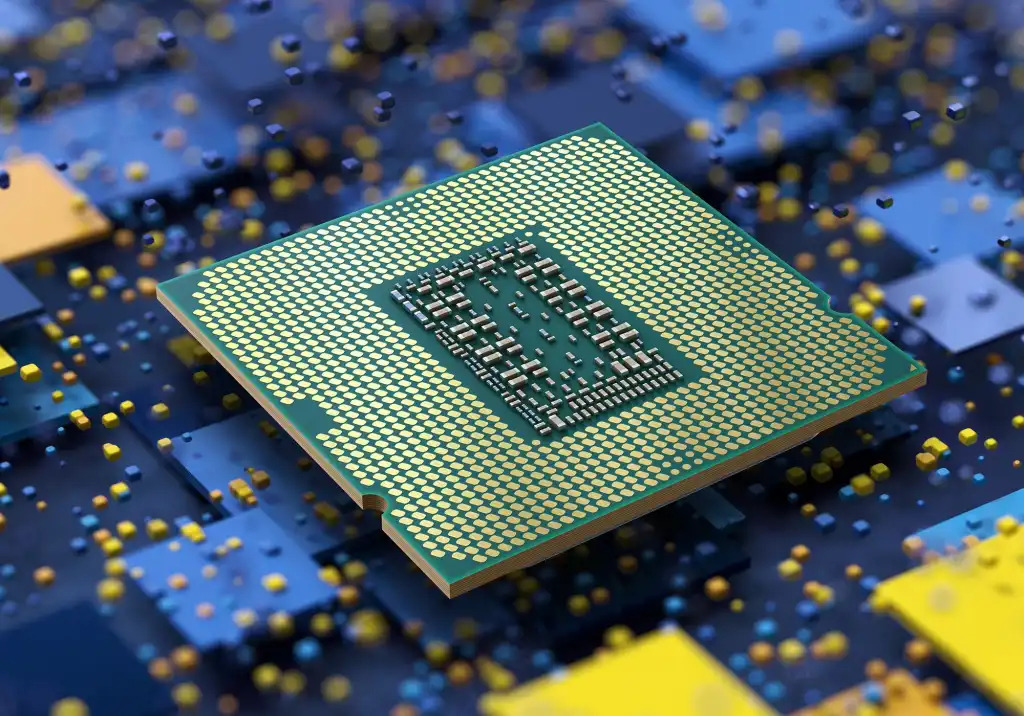
\includegraphics[width=0.6\textwidth]{../misc/cpu.jpg}}

\date{%
    \textit{Parallel and Distributed Computing - Faculdade de Engenharia da Universidade do Porto} \\[2ex]%
    \today
}

{\let\newpage\relax\maketitle}

\clearpage
\setcounter{page}{1}

\pagebreak

\tableofcontents

\begin{abstract}

    In this project, we'll look into how memory hierarchy affects CPU efficiency when processing big volumes of data.

    For that, we're using 3 different algorithms to multiply matrices, and we're comparing their performance. We explain each of the algorithm and how
    they work, on section \ref{Problem Description and Algorithms Explanation}.

    On section \ref{Performance metrics}, we present the harware counters, provided by the Performance API (PAPI), that we used to measure the performance
    of the algorithms, cache and cpu-wise. We also expalin what each of the counters means.

    We also evaluate each algorithm perfomance by measuring the time it takes to run: each one was run 12 times, and the best and worst results were discarded.
    There are clearly improvements in the perfomance of the second algorithm, compared to the first one, but the third one is the one that performs the best.

    On section \ref{FLOPS} we present the Floating Point Operations Per Second (FLOPS) of each algorithm, and on section \ref{Counters} we present the results of the counters.

    Finally, on section \ref{Conclusion}, we conclude the project.


\end{abstract}

\pagebreak
\pagenumbering{arabic}

\section{Problem Description and Algorithms Explanation}\label{Problem Description and Algorithms Explanation}

This project aims to study how memory hierarchy affects CPU efficiency when processing large volumes of data, specifically through
the case study of matrix multiplication.

Performance indicators will be gathered using the Performance API.

Understanding the memory hierarchy's impact is essential to optimize system performance when dealing with large datasets.

The research aims to provide insights into the effectiveness of memory hierarchy in accessing large datasets and improve system performance
and resource utilization.

To assess that impact, we'll use three different algorithms to multiply matrices, and we'll compare their performance:normal matrix multiplication, line*line matrix multiplication, and block multiplication.

\subsection{First Algorithm}\label{First Algorithm}

The "basic" matrix multiplication algorithm is the standard approach that multiplies one line of the first matrix by each column of the second matrix.


\begin{figure}[H]
    \centering
    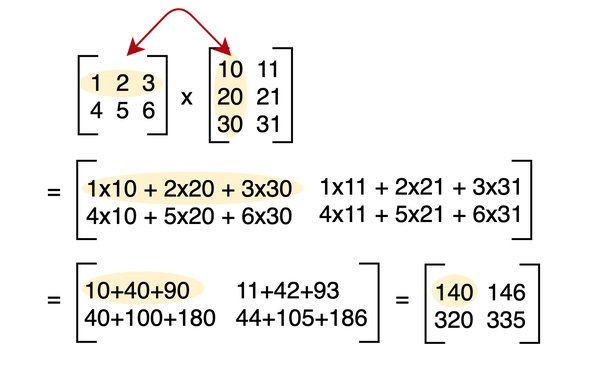
\includegraphics[width=0.4\linewidth]{../misc/main-qimg-9f4bc453b30ef200197f0a1b894df305-pjlq.jpg}
    \caption{Standard Matrix Multiplication Algorithm}
\end{figure}

\subsection{Second Algorithm}\label{Second Algorithm}

The line*line matrix multiplication algorithm is a variant that multiplies an element from the first matrix by the correspondent line of the second matrix.

\begin{figure}[H]
    \centering
    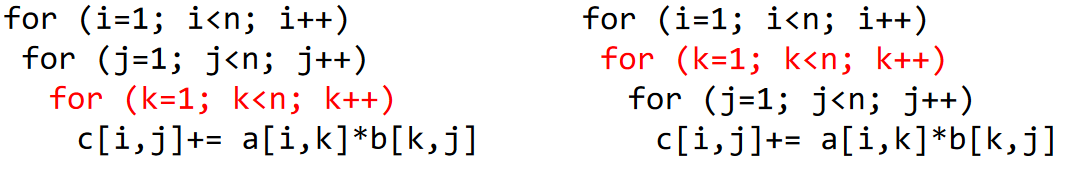
\includegraphics[width=0.4\linewidth]{../misc/linevsnormal.png}
    \caption{On the left, the standard multiplication process. On the right, the line variant.}
\end{figure}

\subsection{Third Algorithm}\label{Third Algorithm}

The block multiplication, is a block oriented algorithm that divides the matrices in blocks and uses the
same sequence of computation as in the line*line algorithm.

\begin{figure}[H]
    \centering
    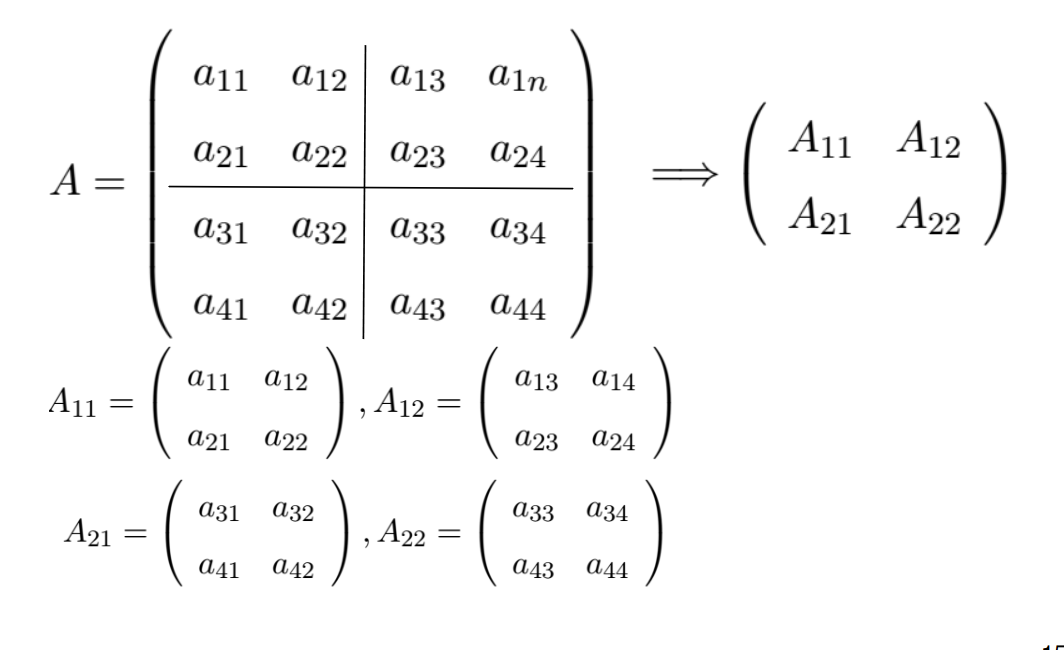
\includegraphics[width=0.4\linewidth]{../misc/block-matrix.png}
    \caption{Matrix Multiplication with the Block Technique}
\end{figure}



\section{Performance metrics}\label{Performance metrics}

The algorithms have been tested with different matrix dimensions, and after running each algorithm 12 times,
we removed the best and worst performance results and calculated the average time it took to run.
This approach helps to reduce the impact of outliers and provides a more accurate representation of
the typical performance of each algorithm.

To assess the hardware performance of the algorithms, we used the Performance API (PAPI) to gather performance indicators.

Out of the 59 hardware performance counters\footnote{Available on FEUP's computer}, provided by the PAPI API, we chose to thorough analyze the following:

\begin{table}[H]
    \centering
    \begin{tabular}{|l|l|l|}
        \hline
        \textbf{Identifier}                        & \textbf{Derived} & \textbf{Description}                              \\ \hline
        PAPI\textunderscore L1\textunderscore DCM  & Yes              & L1 instruction cache misses                       \\ \hline
        PAPI\textunderscore L2\textunderscore DCA  & No               & L2 data cache accesses                            \\ \hline
        PAPI\textunderscore L3\textunderscore DCA  & Yes              & L3 data cache accesses                            \\ \hline
        PAPI\textunderscore TOT\textunderscore CYC & Yes              & Total cycles                                      \\ \hline
        PAPI\textunderscore TOT\textunderscore INS & No               & Total instructions                                \\ \hline
        PAPI\textunderscore TLB\textunderscore DM  & Yes              & Data translation lookaside buffer misses          \\ \hline
        PAPI\_CA\_CLN                              & No               & Requests for exclusive access to clean cache line \\ \hline
    \end{tabular}
    \caption{Hardware Performance Counters}
\end{table}

\textbf{PAPI\textunderscore L1\textunderscore ICM}  measures the number of instruction cache misses in the CPU. The instruction cache is a small memory
that stores the instructions that the CPU will execute.
This counter is useful for identifying CPU-related performance issues.

\textbf{PAPI\textunderscore L2\textunderscore DCA} measures the number of data cache accesses in the CPU. Useful for cache-related performance issues.

\textbf{PAPI\textunderscore L3\textunderscore DCA} measures the number of data cache accesses in the CPU. Useful for cache-related performance issues.

\textbf{PAPI\textunderscore TOT\textunderscore CYC} measures the number of CPU cycles . A CPU cycle is the time it takes for the CPU to complete one instruction. This counter is useful for identifying CPU-related performance issues.

\textbf{PAPI\textunderscore TOT\textunderscore INS} measures the number of instructions in the CPU. Used to identify CPU-related performance issues.

\textbf{PAPI\textunderscore TLB\textunderscore DM} the metric counts the instances when the CPU encounters a data TLB miss, which happens when the TLB cache doesn't have the required data for a memory access. This results in the CPU accessing main memory,
which can be slow, and the metric helps identify performance issues related to data TLB.


\vspace{20px}

We've also computed the floating-point operations per second (\textbf{FLOPS})


\section{Results and Analysis}\label{Results and Analysis}

\subsection{Exercise 1}\label{Exercise 1}

On the first exercise, we set "lower bound" of how the algorithms should behave perfomance-wise. This is due to the fact that this algorithm is deemed the "normal" approach to matrix multiplication, without any optimizations, which results in the least
efficient algorithm.

As mentioned before, the algorithm was developed in both C++ and Java, and were tested for matrix sizes from 600 to 3000,
with a step of 400. The results are shown in the following figure.

\begin{figure}[H]
    \centering
    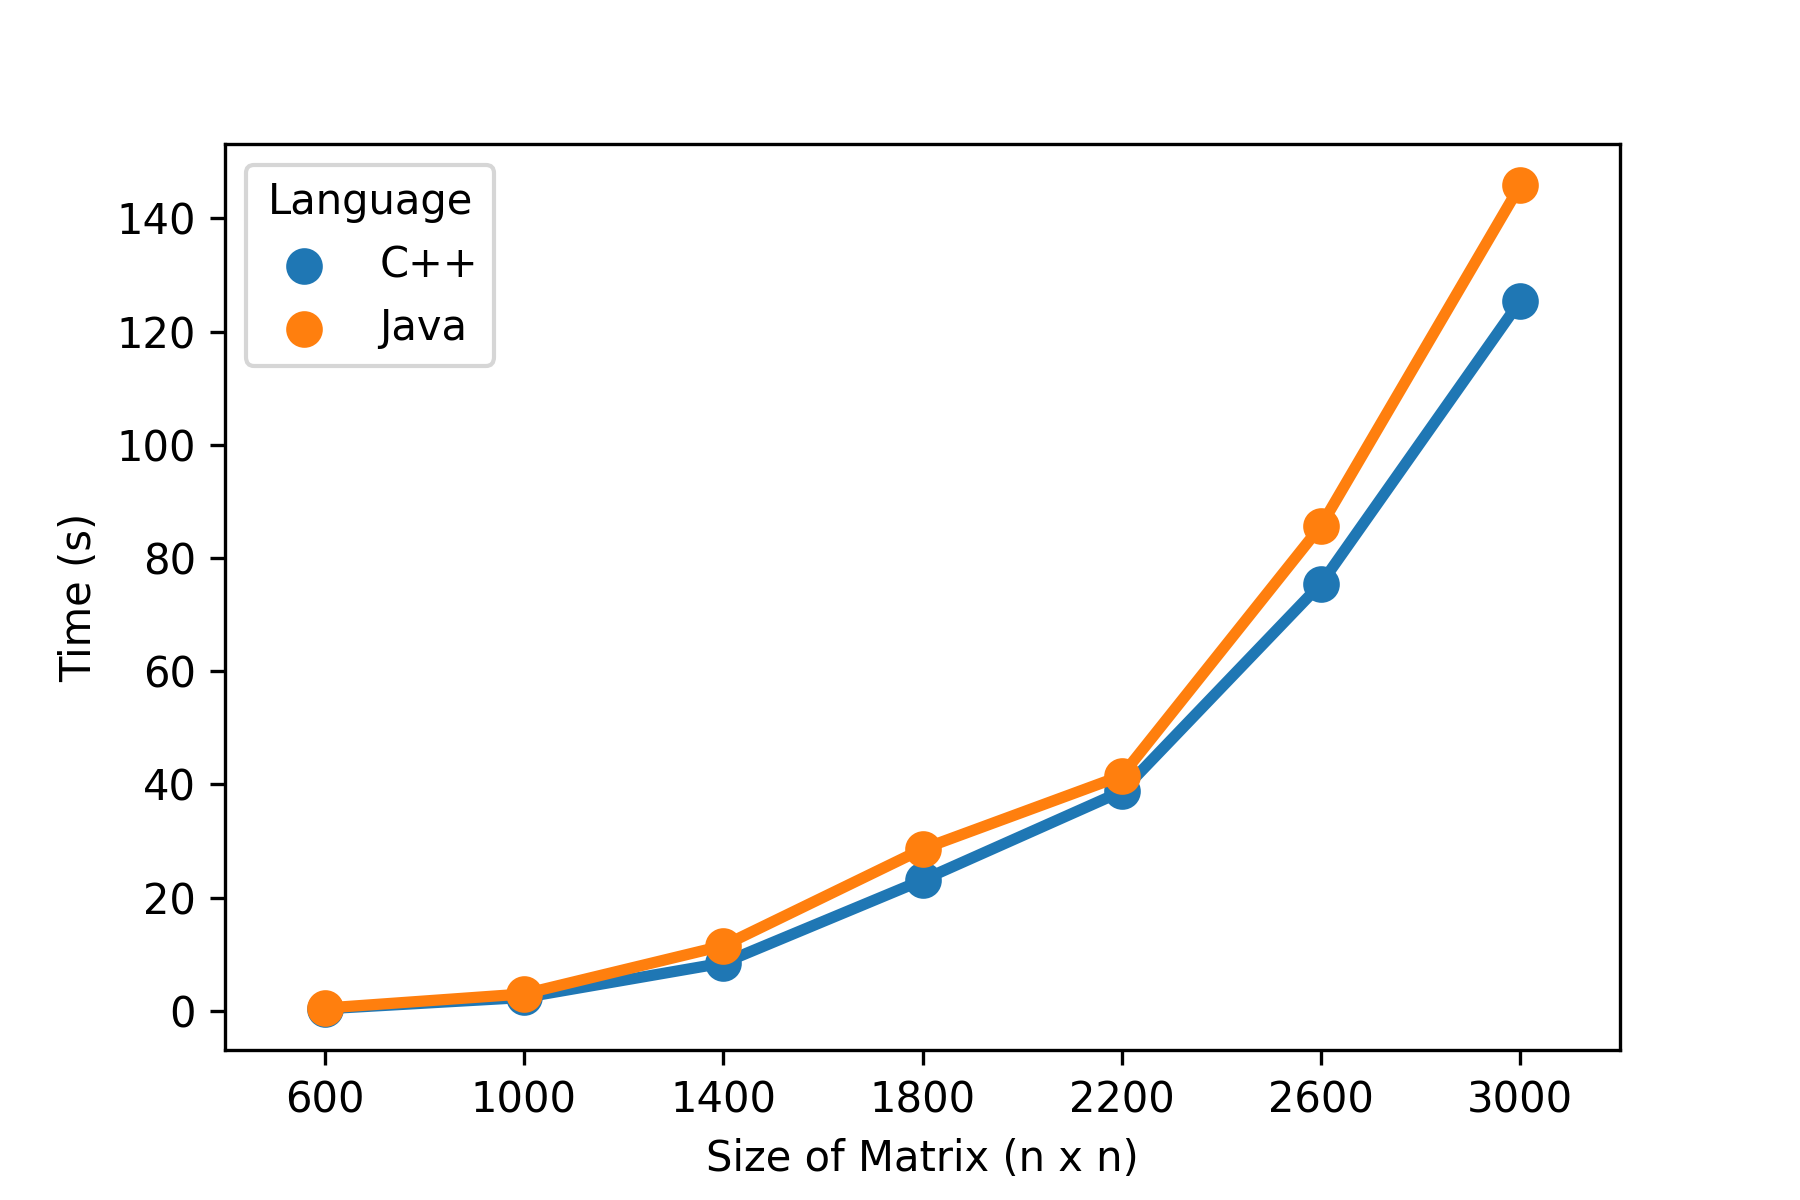
\includegraphics[width=0.5\linewidth]{../plots/ex1/ex1-overall.png}
    \caption{Ex.1 - C++ vs Java average runtime with different matrix sizes}
\end{figure}

As we can see from the figure, the C++ implementation is slightly faster than the Java one, but the difference is not significant
enough to be considered relevant until we reach the 2600x2600 matrix size, where the Java version takes 10 seconds longer to run. That difference climbs to
20 seconds when we reach the 3000x3000 matrix size.
\par
In general, C++ is often considered a faster language than Java due to a number of factors.
C++ allows for more low-level memory management, which can allow for more efficient use of resources.
C++ also compiles directly to machine code, whereas Java code runs on a virtual machine,
which can introduce some overhead.


\subsection{Exercise 2}\label{Exercise 2}

On the second exercise, a line approach was taken to the problem, which resulted in a more efficient algorithm.
The algorithm was developed in both C++ and Java, and were tested for matrix sizes from 600 to 3000, with a step of 400.
The results are shown in the following figure.

\begin{figure}[H]
    \centering
    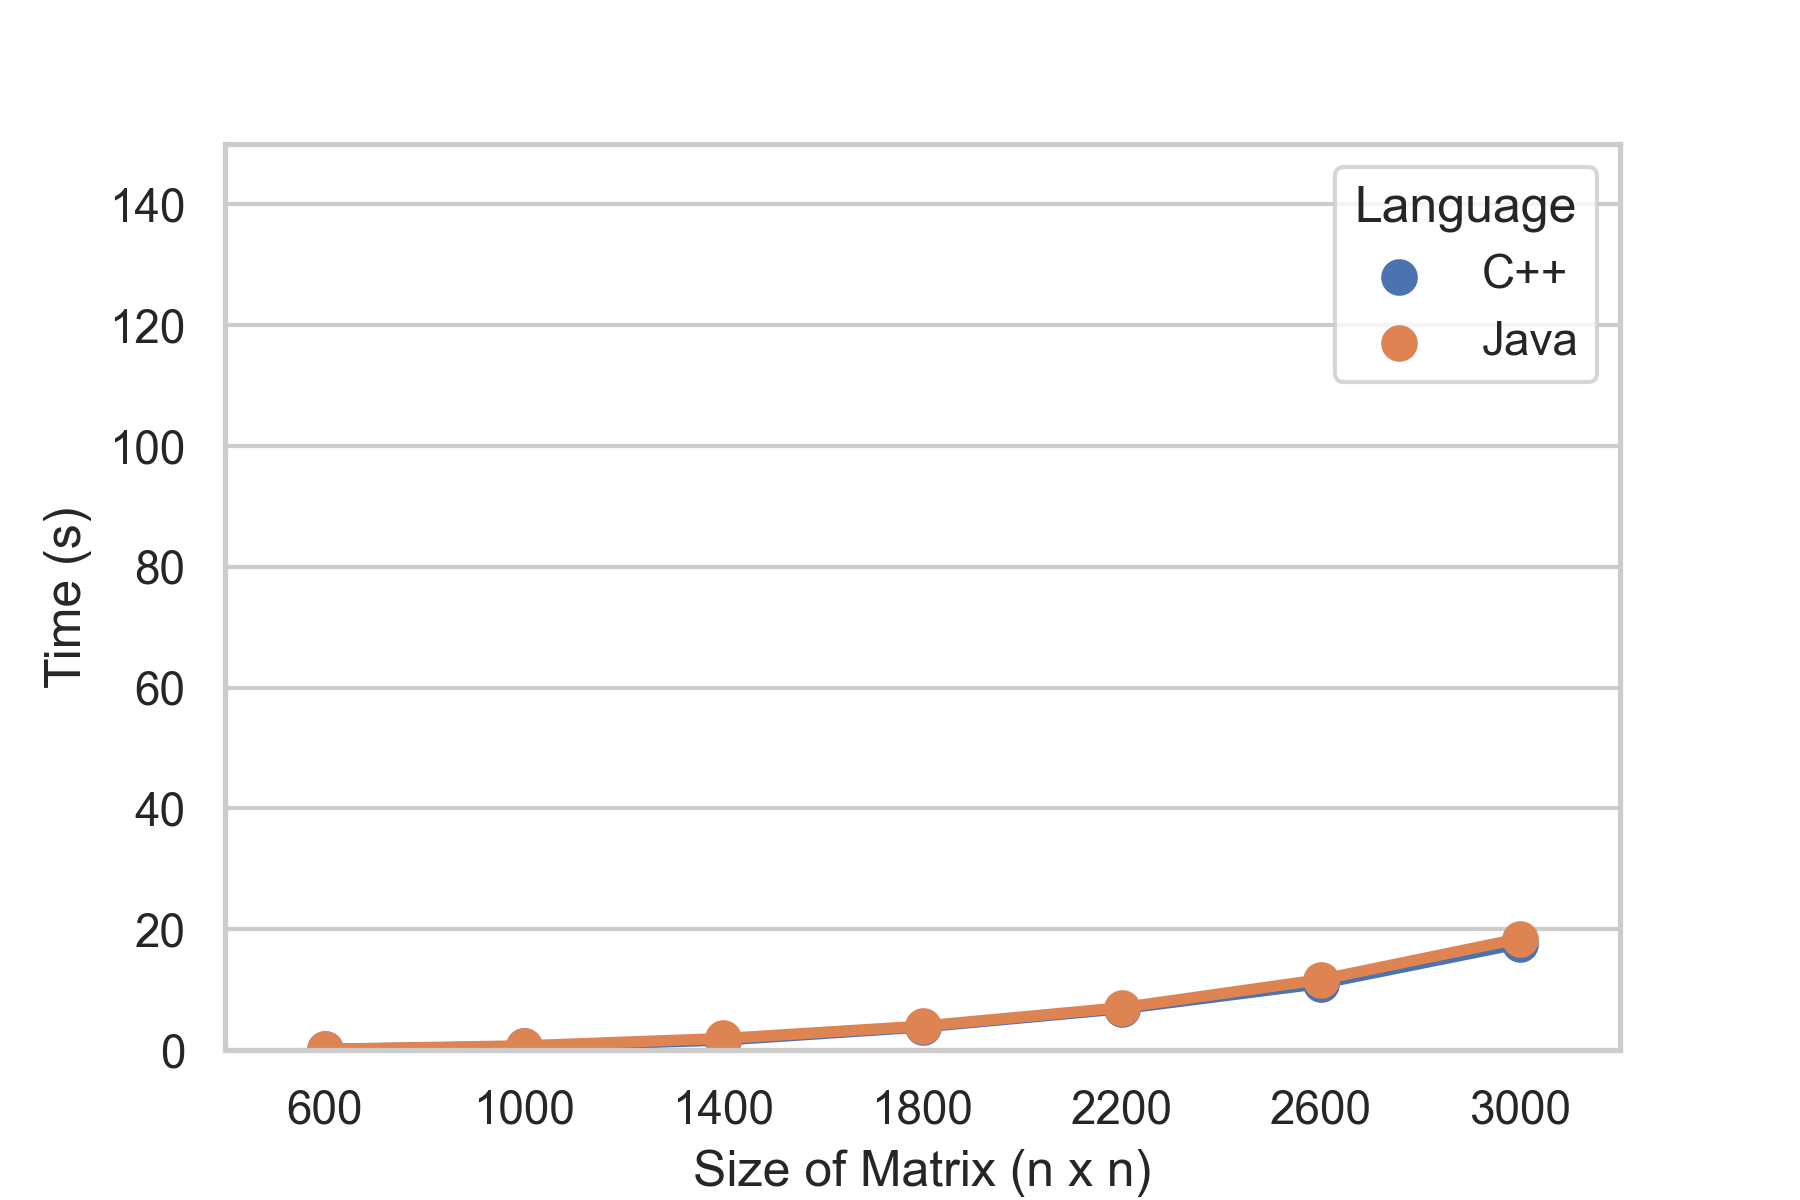
\includegraphics[width=0.5\linewidth]{../plots/ex2/ex2a-overall.png}
    \caption{Ex.2 - C++ vs Java average runtime with different matrix sizes}
    \label{ex2-overall}
\end{figure}

On figure \ref{ex2-overall}, we see that we've implemented a way more efficient algorithm. For the matrix size of 1800x1800, the optimized variant
is about 20 seconds faster. For the 3000x3000 matrix size, this number is around 100 seconds, which is a significant improvement.

It's also visible that the differences between the C++ and Java implementations are not as significant as in the
previous implementation, with the C++ version being only 0.8 seconds faster than the Java one for the 3000x3000 matrix size.


To futher visualize the improvement, the following figure contains both plots, side by side.
\begin{figure}[H]
    \centering
    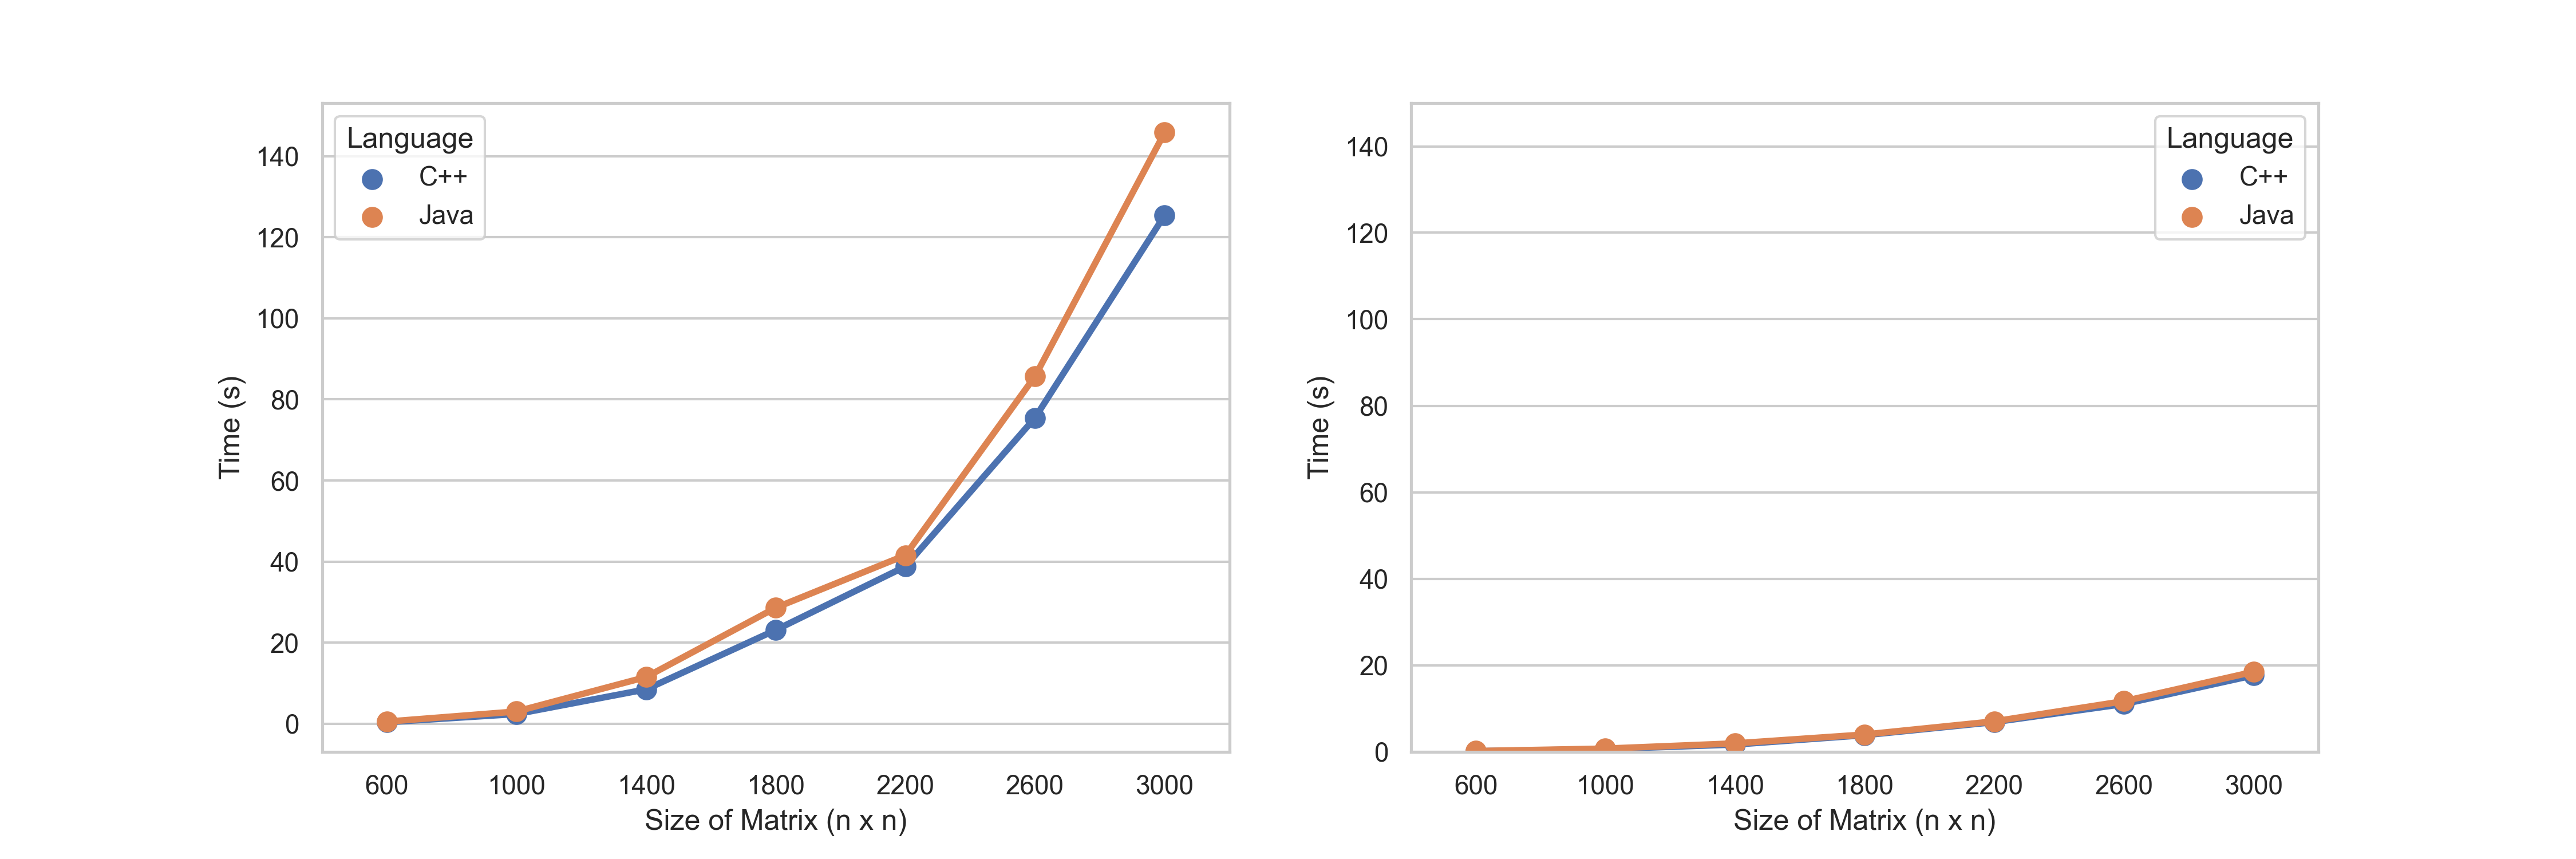
\includegraphics[width=.9\linewidth]{../plots/ex1-ex2a-overall.png}
    \caption{Exercise 1 vs Exercise 2 Performance Comparison}
    \label{ex2-overall2}
\end{figure}


\vspace*{20px}

We were also tasked with running the second algorithm's C++ implementation with higher matrix sizes, to see how it would behave.
The algorithm was tested for matrix sizes from 4096 to 10240, with a step of 2048. The results are shown in the following figure.

\begin{figure}[H]
    \centering
    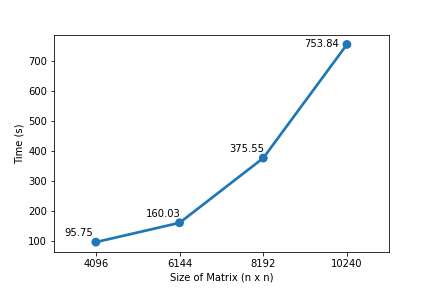
\includegraphics[width=0.5\linewidth]{../plots/ex2/ex2_higher.png}
    \caption{Ex.2 - C++ average runtime with higher matrix sizes}
\end{figure}

\subsection{Exercise 3}\label{Exercise 3}

On the third and last exercise, we've implemented a variant that splits the matrix into blocks, and then multiplies them.
The algorithm was developed in C++ and was tested for matrix sizes from 4096 to 10240, with a step of 2048.
Each size was tested with a block size that ranges from 128 to 512, with a step of 128.

The following image shows the average time it took to run the algorithm for the matrix of size 4096x4096,
with different block sizes.

\begin{figure}[H]
    \centering
    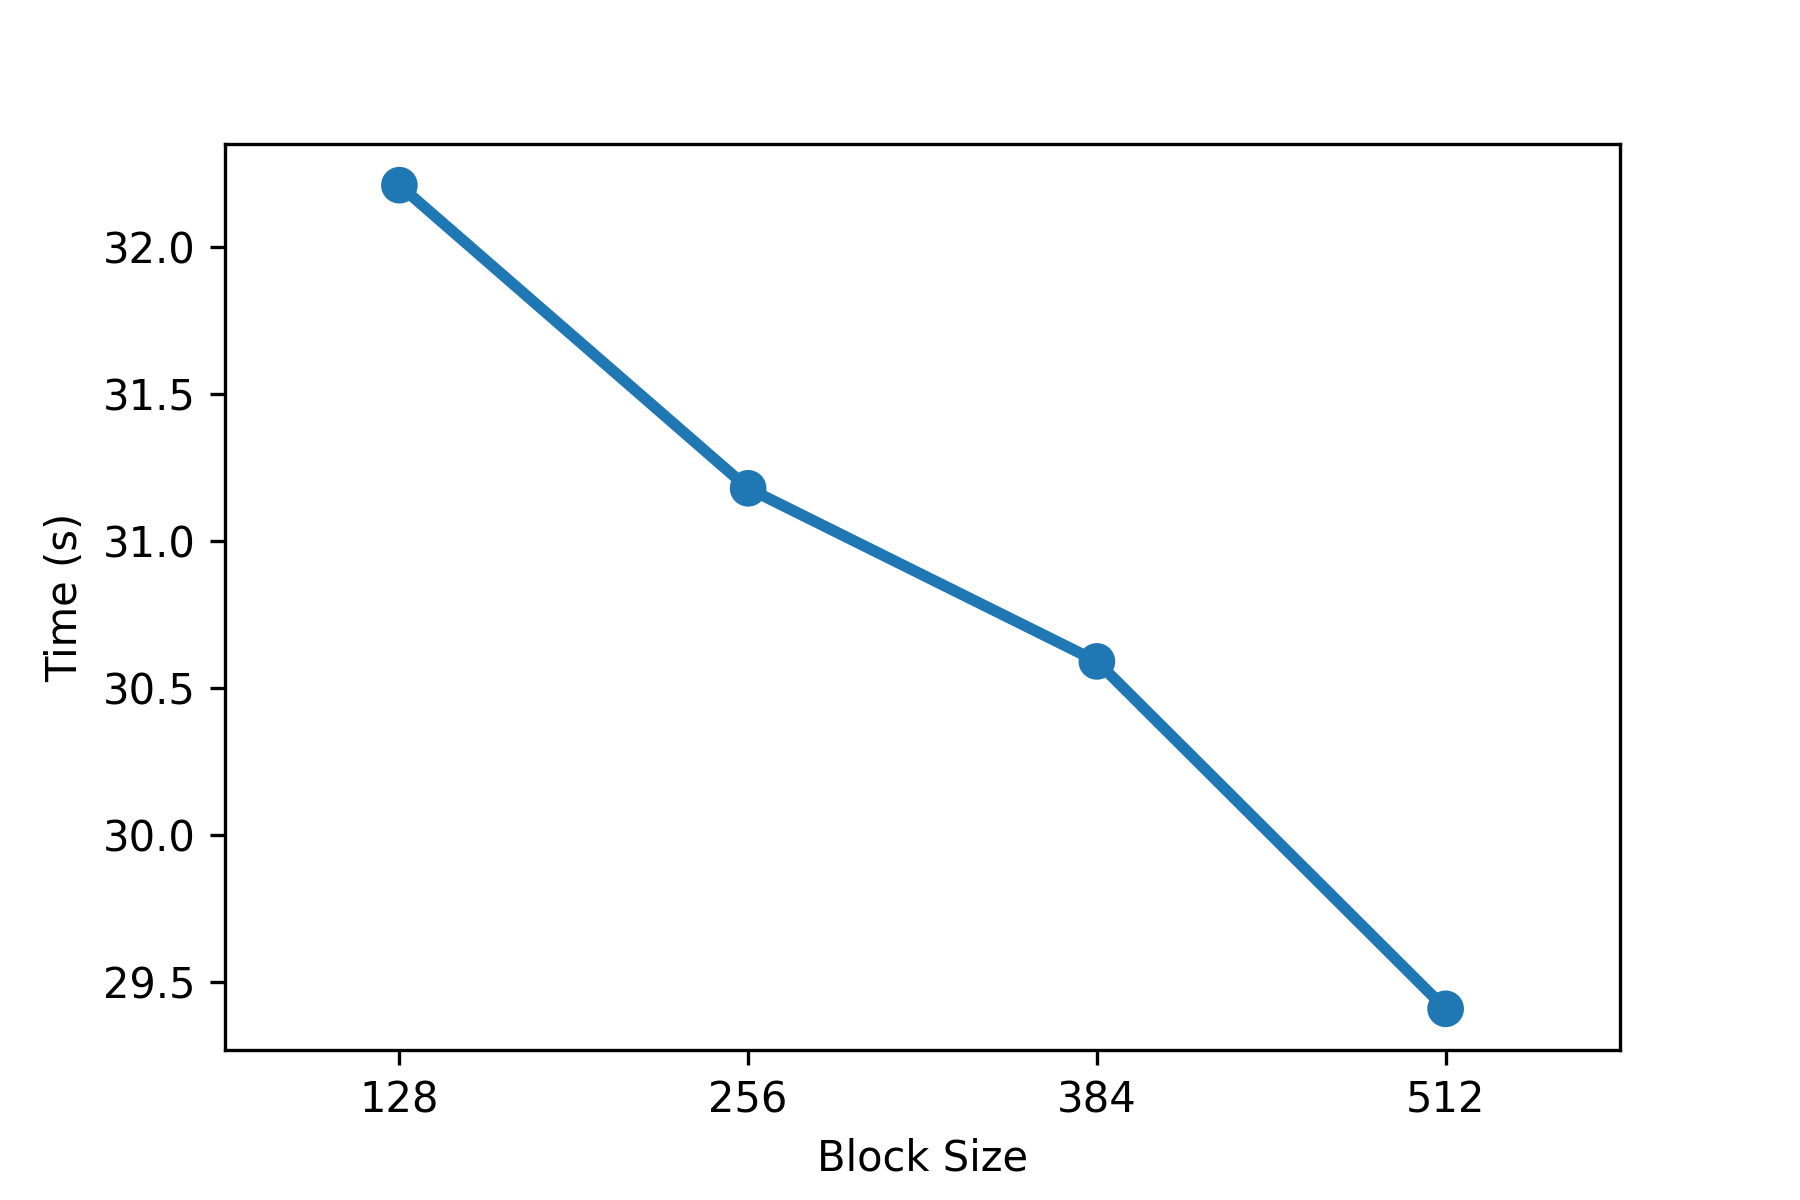
\includegraphics[width=0.5\linewidth]{../plots/ex3/ex3-4096.png}
    \caption{Ex.3 - C++ average runtime with different block sizes for a 4096x4096 matrix}
\end{figure}

From observing the figure, we can see that the algorithm's performance gets better as the block size increases.
We speculated that this would also apply to the other matrix sizes, and was proven correct, as the following image shows.

The image below describes the overall picture of the algorithm's performance, with different matrix sizes and block sizes.

\begin{figure}[H]
    \centering
    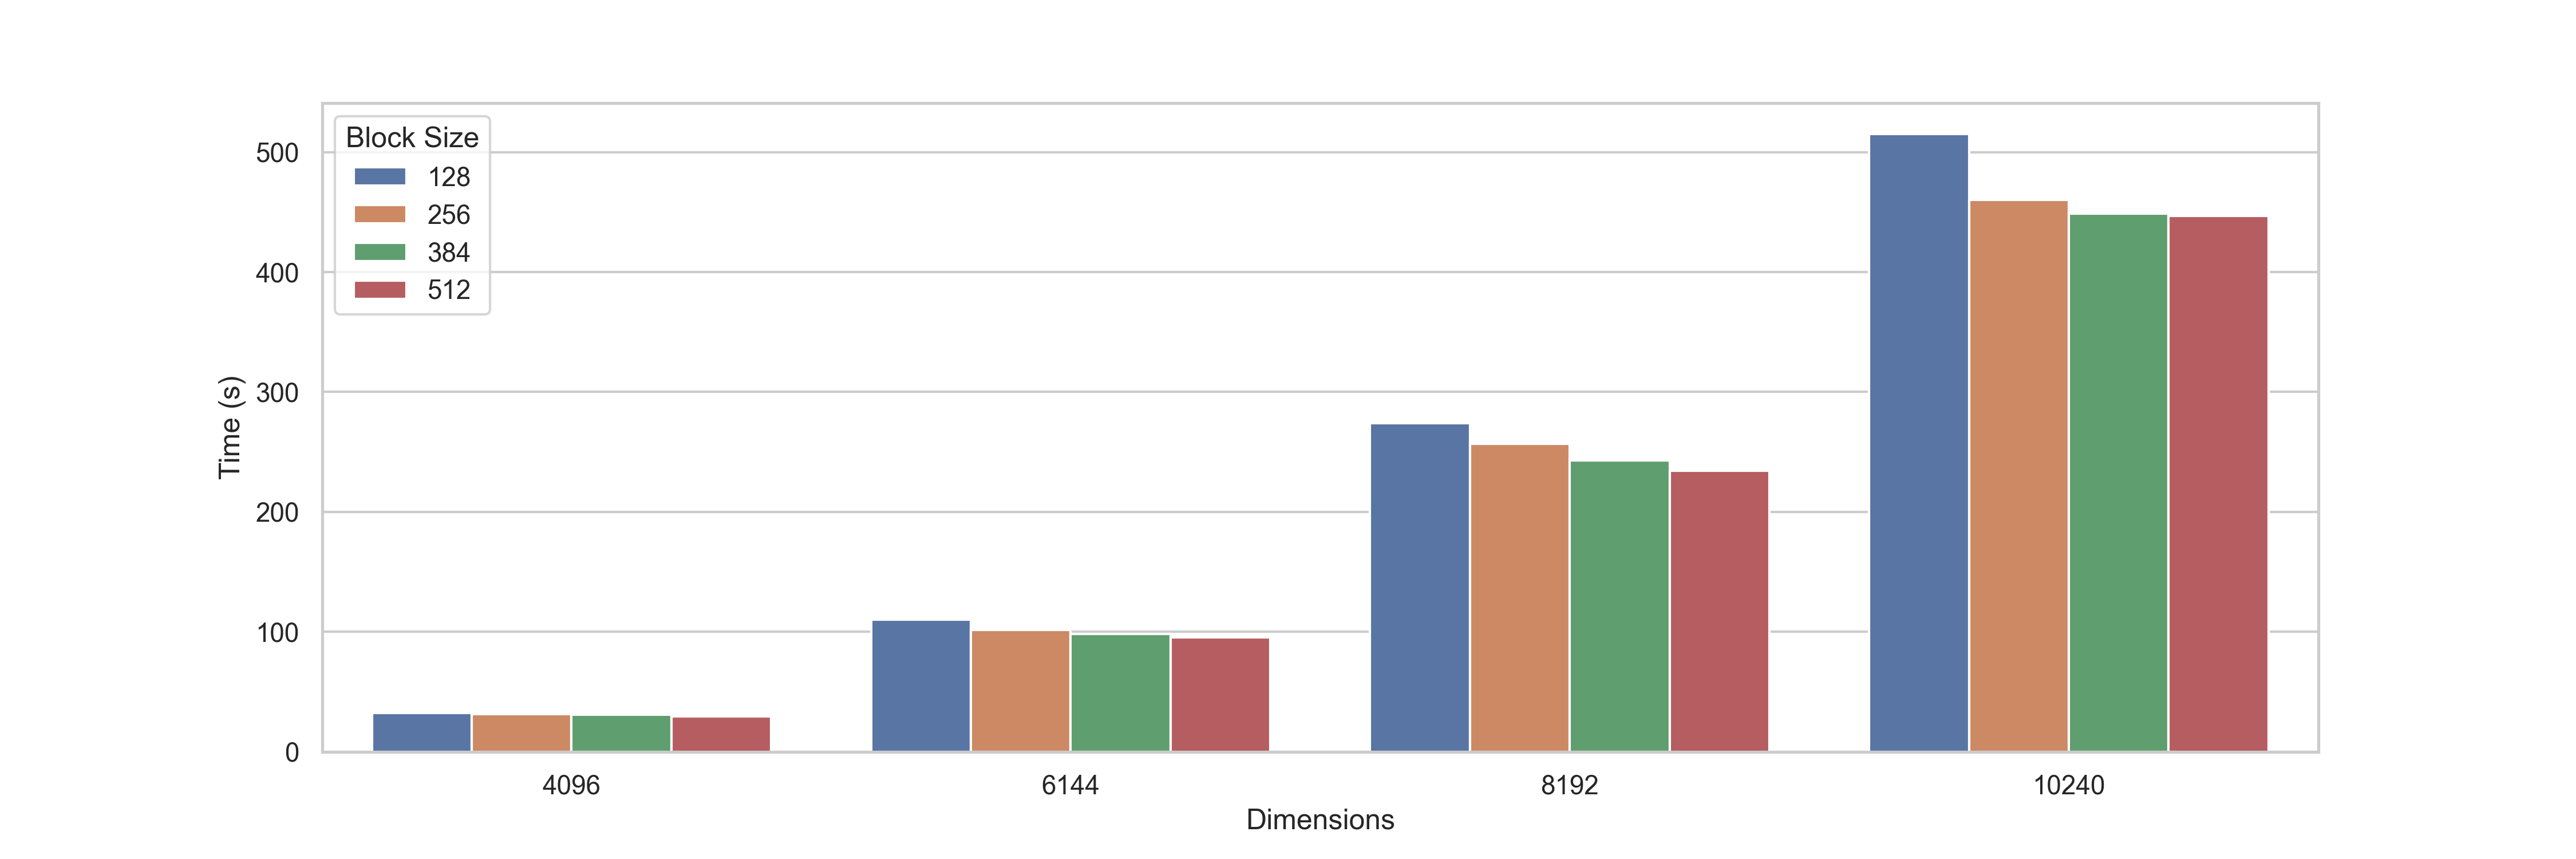
\includegraphics[width=\linewidth]{../plots/ex3/ex3-overall.png}
    \caption{Ex.3 - C++ average runtime with different matrix sizes and block sizes}
\end{figure}

As we can prove from the figure, the algorithm's performance gets better as the block size increases, for every matrix size.
The best performance was achieved with a block size of 512, which was at least 10\% faster than the 128 block size.

\vskip 20pt

To assess the perfomance of this matrix multiplication algorithm variant, we analysed it against the second variant,
which was, until now, the most efficient one.

\begin{figure}[H]
    \centering
    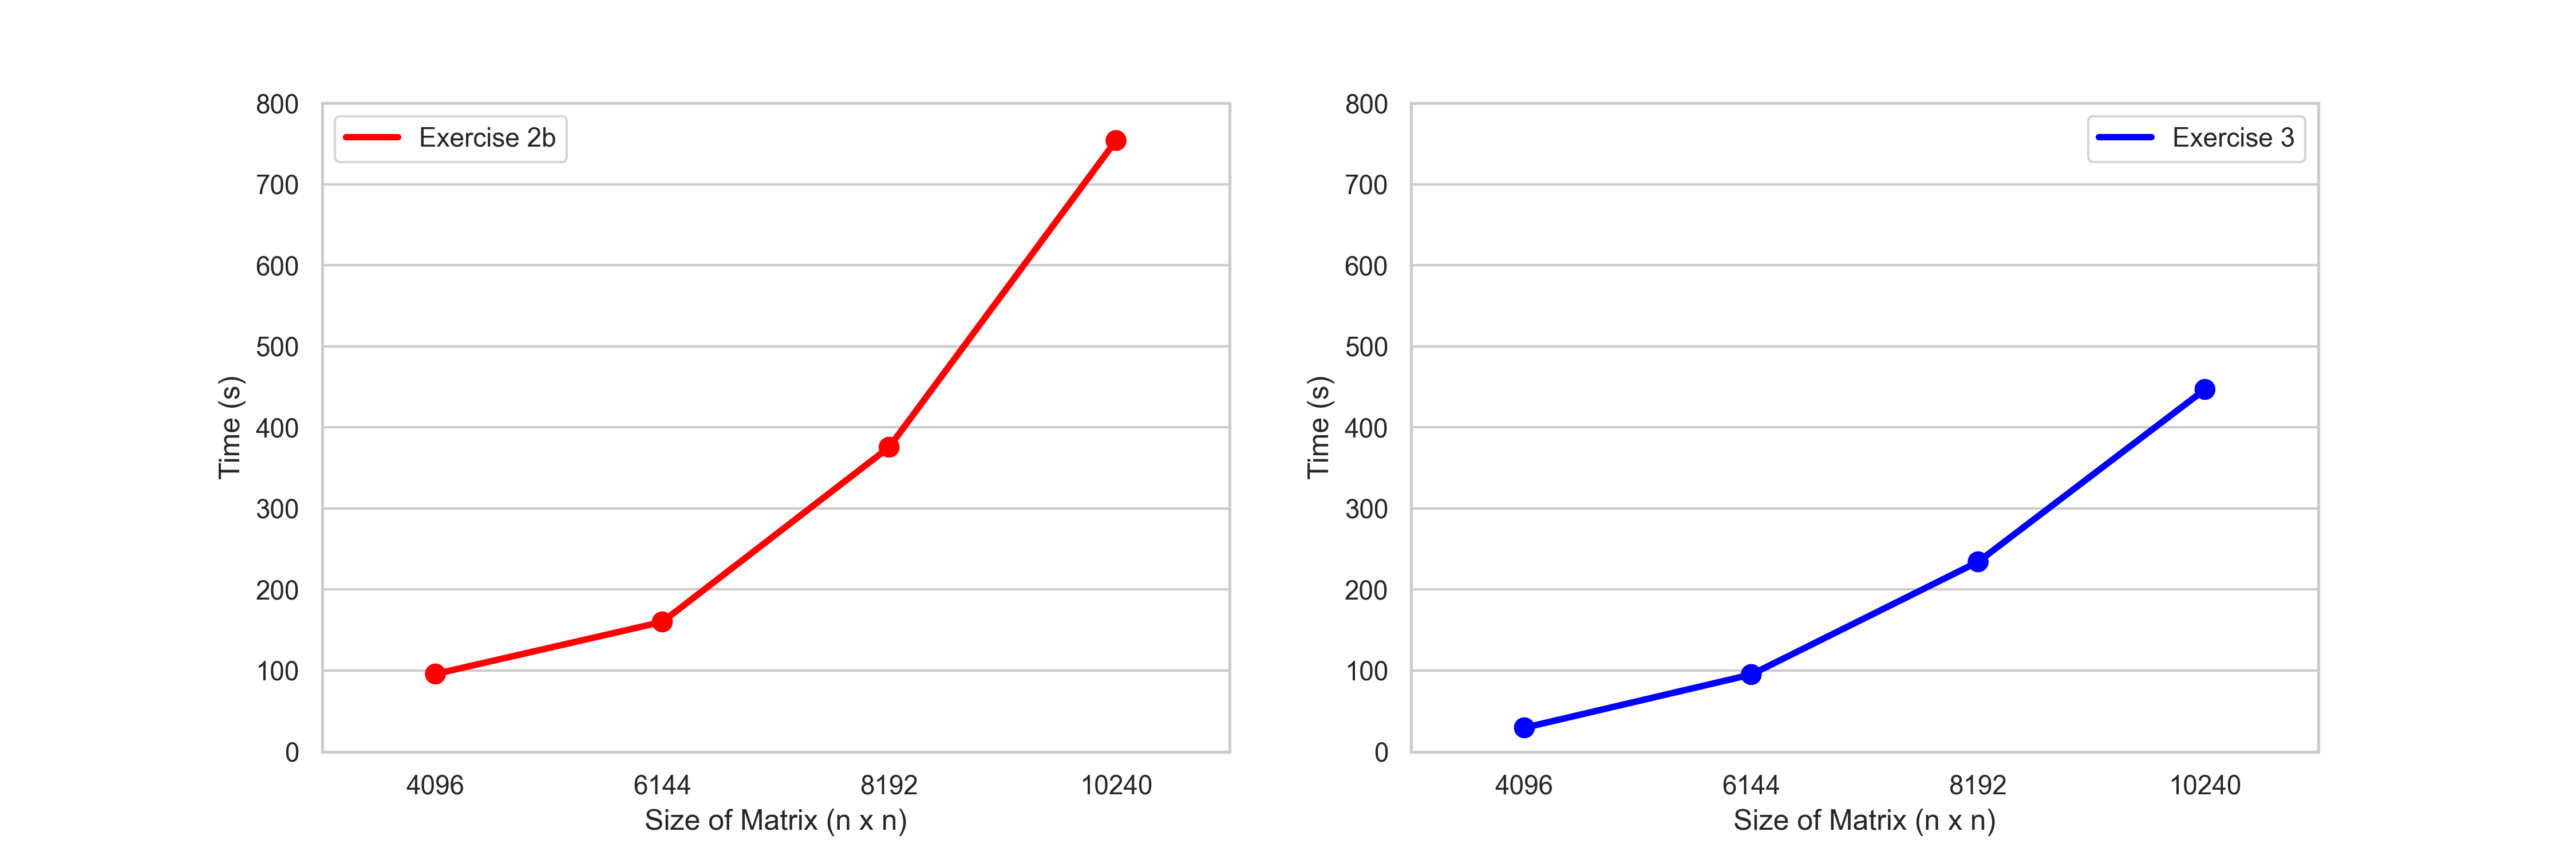
\includegraphics[width=.9\linewidth]{../plots/ex2b-ex3-overall.png}
    \caption{Exercise 2 vs Exercise 3 Performance Comparison}
    \label{ex3-overall}
\end{figure}

From the image above, we see that the third variant is indeed the most efficient.

\subsection{Counters}\label{Counters}

For the first and second exercises, we were able to retrieve all the counters that we were set to, as we had the time to run
the algorithms on the university's computers. For the third exercise, we were only able to retrieve Level 1 and Level 2 instruction cache misses
and level 2 data cache misses.

In the following table:

\begin{table}[H]
    \centering
    \begin{tabular}{|c|c|c|}
        \hline
        \textbf{Counter} & \textbf{Exercise 1} & \textbf{Exercise 2a} \\ \hline
        PAPI\_L1\_DCM    & 3515069772          & 345713540            \\ \hline
        PAPI\_L2\_DCA    & 140029979750792     & 140072199426440      \\ \hline
        PAPI\_L3\_DCA    & 2                   & 2                    \\ \hline
        PAPI\_TOT\_CYC   & 140029979797440     & 140072199473088      \\ \hline
        PAPI\_TOT\_INS   & 140723630164368     & 140728093170256      \\ \hline
        PAPI\_CA\_CLN    & 290339              & 507                  \\ \hline
    \end{tabular}
    \caption{Counter Comparison for 1400x1400 Matrix Size}
\end{table}

In the table above, the following conclusions were made:
\begin{itemize}
    \item The L1 data cache misses are much higher on the first exercise, being around 10 times higher: The first algorithm had 3 billion
          cache misses, while the second one had only 345 million.
    \item The first algorithm had 290 thousand cache lines cleaned, while the second one had only 507. This is an important measure, since the second algorithm takes advantage
          of the way that the matrix is stored in memory, while the first one is constatly cleaning the cache lines and reloading them with new data.
\end{itemize}Requests for exclusive access to clean cache line yap

As mentioned before, for the last exercise, we were only able to retrieve the L1 and L2 instruction cache misses and level 2 data cache misses.
The following table shows the comparision between all the 3 implementations:

\begin{table}[H]
    \centering
    \begin{tabular}{|c|c|c|c|}
        \hline
        \textbf{Counter} & \textbf{Exercise 1} & \textbf{Exercise 2a} & \textbf{Exercise 3} \\ \hline
        PAPI\_L1\_ICM    & 6159                & 7133                 & 192844              \\ \hline
        PAPI\_L2\_DCM    & 1039265512          & 690672335            & 46268402            \\ \hline
        PAPI\_L2\_ICM    & 5368                & 4160                 & 9650501             \\ \hline
    \end{tabular}
    \caption{Counter Comparison for 1400x1400 Matrix Size}
\end{table}

From the table above, we see that the third algorithm has a substantially higher number of both L1 and L2 instruction cache misses. This is due to the fact that the algorithm
uses a lot of pointers, which are stored in the cache, and are constantly being accessed.
This is a problem, since the cache is not big enough to store all the pointers, and the algorithm has to constantly reload them from memory.

However, we also conclude that it has significantly less L2 data cache misses, indicating a better data locality.

\subsection{FLOPS}\label{FLOPS}

The ammount of flops was calculated by dividing the ammount of operations of the algorithms by the time it took to run them.
We used the averages of the GFlops for the different matrix sizes.

The results are shown below:

\begin{itemize}
    \item Exercise 1
          \begin{itemize}
              \item \textbf{C++} - 1.2 GFlops/s
              \item \textbf{Java} - 0.9 GFlops/s
          \end{itemize}
    \item Exercise 2a
          \begin{itemize}
              \item \textbf{C++} - 5.12 GFlops/s
              \item \textbf{Java} - 4.44 GFlops/s
          \end{itemize}
    \item Exercise 2b
          \begin{itemize}
             \item   \textbf{C++} - 3.79 GFlops/s
          \end{itemize}
    \item Exercise 3
          \begin{itemize}
              \item \textbf{C++} - 6.2 GFlops/s
          \end{itemize}
\end{itemize}


\section{Conclusions}\label{Conclusion}

Overall, the evidence presented in this report supports the idea that optimizing our algorithms to take advantage of the way the data is stored in memory
can lead to a significant performance improvement. While the first algorithm implemented a naive and straightforward approach,
the second and third algorithms took advantage of that, and we were to achieve significant better results in terms of performance.

We believe that the project goals were achieved, and that the results presented in this report are conclusive.

We were able to grasp concepts such as data locality, cache hit/miss, cache line cleaning.

If time were not a factor, we would have liked to take a deep dive into the PAPI counters, and find interesting insights about the way the algorithms were running.

\quad


\clearpage
\pagenumbering{gobble}

\begin{appendices}

    \section{Hardware Used}\label{Hardware Used}

    We used two different machines to run the tests, one was used to run the algorithm 12 times each and
    compute the average time, and the other, a linux machine, was used to run the PAPI counters.

    \begin{lstlisting}[caption={Linux Machine System Information},label={lst:sys_info}, style=myStyle]
    PAPI version : 7.0.0.0
    Operating system : Linux 5.15.0-58-generic
    Vendor string and code : GenuineIntel (1, 0x1)
    Model string and code : Intel(R) Core(TM) i7-9700 CPU @ 3.00GHz (158, 0x9e)
    CPU revision : 13.000000
    CPUID : Family/Model/Stepping 6/158/13, 0x06/0x9e/0x0d
    CPU Max MHz : 4700
    CPU Min MHz : 800
    Total cores : 8
    SMT threads per core : 1
    Cores per socket : 8
    Sockets : 1
    Cores per NUMA region : 8
    NUMA regions : 1
    Running in a VM : no
    Number Hardware Counters : 10
    Max Multiplex Counters : 384
    Fast counter read (rdpmc): yes

    Memory Cache and TLB Hierarchy Information.
    ------------------------------------------------------------------------
    TLB Information.
    There may be multiple descriptors for each level of TLB
    if multiple page sizes are supported.

    L1 Data TLB:
    Page Size:              4 KB
    Number of Entries:     64
    Associativity:          4

    Cache Information.

    L1 Data Cache:
    Total size:            32 KB
    Line size:             64 B
    Number of Lines:      512
    Associativity:          8

    L1 Instruction Cache:
    Total size:            32 KB
    Line size:             64 B
    Number of Lines:      512
    Associativity:          8

    L2 Unified Cache:
    Total size:           256 KB
    Line size:             64 B
    Number of Lines:     4096
    Associativity:          4

    L3 Unified Cache:
    Total size:         12288 KB
    Line size:             64 B
    Number of Lines:   196608
    Associativity:         12
\end{lstlisting}

    \begin{lstlisting}[caption={Windows Machine System Information},label={lst:win_sys_info}, style=myStyle]
    CPU: Ryzen 5 2700X
    Number of cores: 8
    Number of threads: 16
    RAM: 16GB
    Operating system: Windows 10 Pro 64-bit
    Version: 21H1
    Build: 19043.1348
    L1 cache size: 768KB
    L2 cache size: 4096KB
    L3 cache size: 16384KB
    CPU clock speed: 4.1GHz (overclocked)
    Virtualization: enabled
\end{lstlisting}


\end{appendices}

\end{document}


